\documentclass{beamer}
\usetheme{Boadilla}

\title{Parity Asymmetry in the CMB}
\subtitle{UF REU under Dr. Zachary Slepian}
\author{Michael Bartlett}
\institute{University of Oklahoma}
\date{\today}

\begin{document}

\begin{frame}
    \titlepage
\end{frame}

\begin{frame}
    \frametitle{Outline}
    \tableofcontents
\end{frame}

\section{Overview of the Problem}
\begin{frame}{Overview of the problem}
    The goal is to determine whether or not parity asymmetry can be detected using the Cosmic Microwave Background.
    To do so we are modelling the 4-point correlation function as a function of 4 points on a sphere, defined by vectors $\vec x_0, \vec x_1, \vec x_2, \vec x_3$
    \begin{figure}
        \centering
        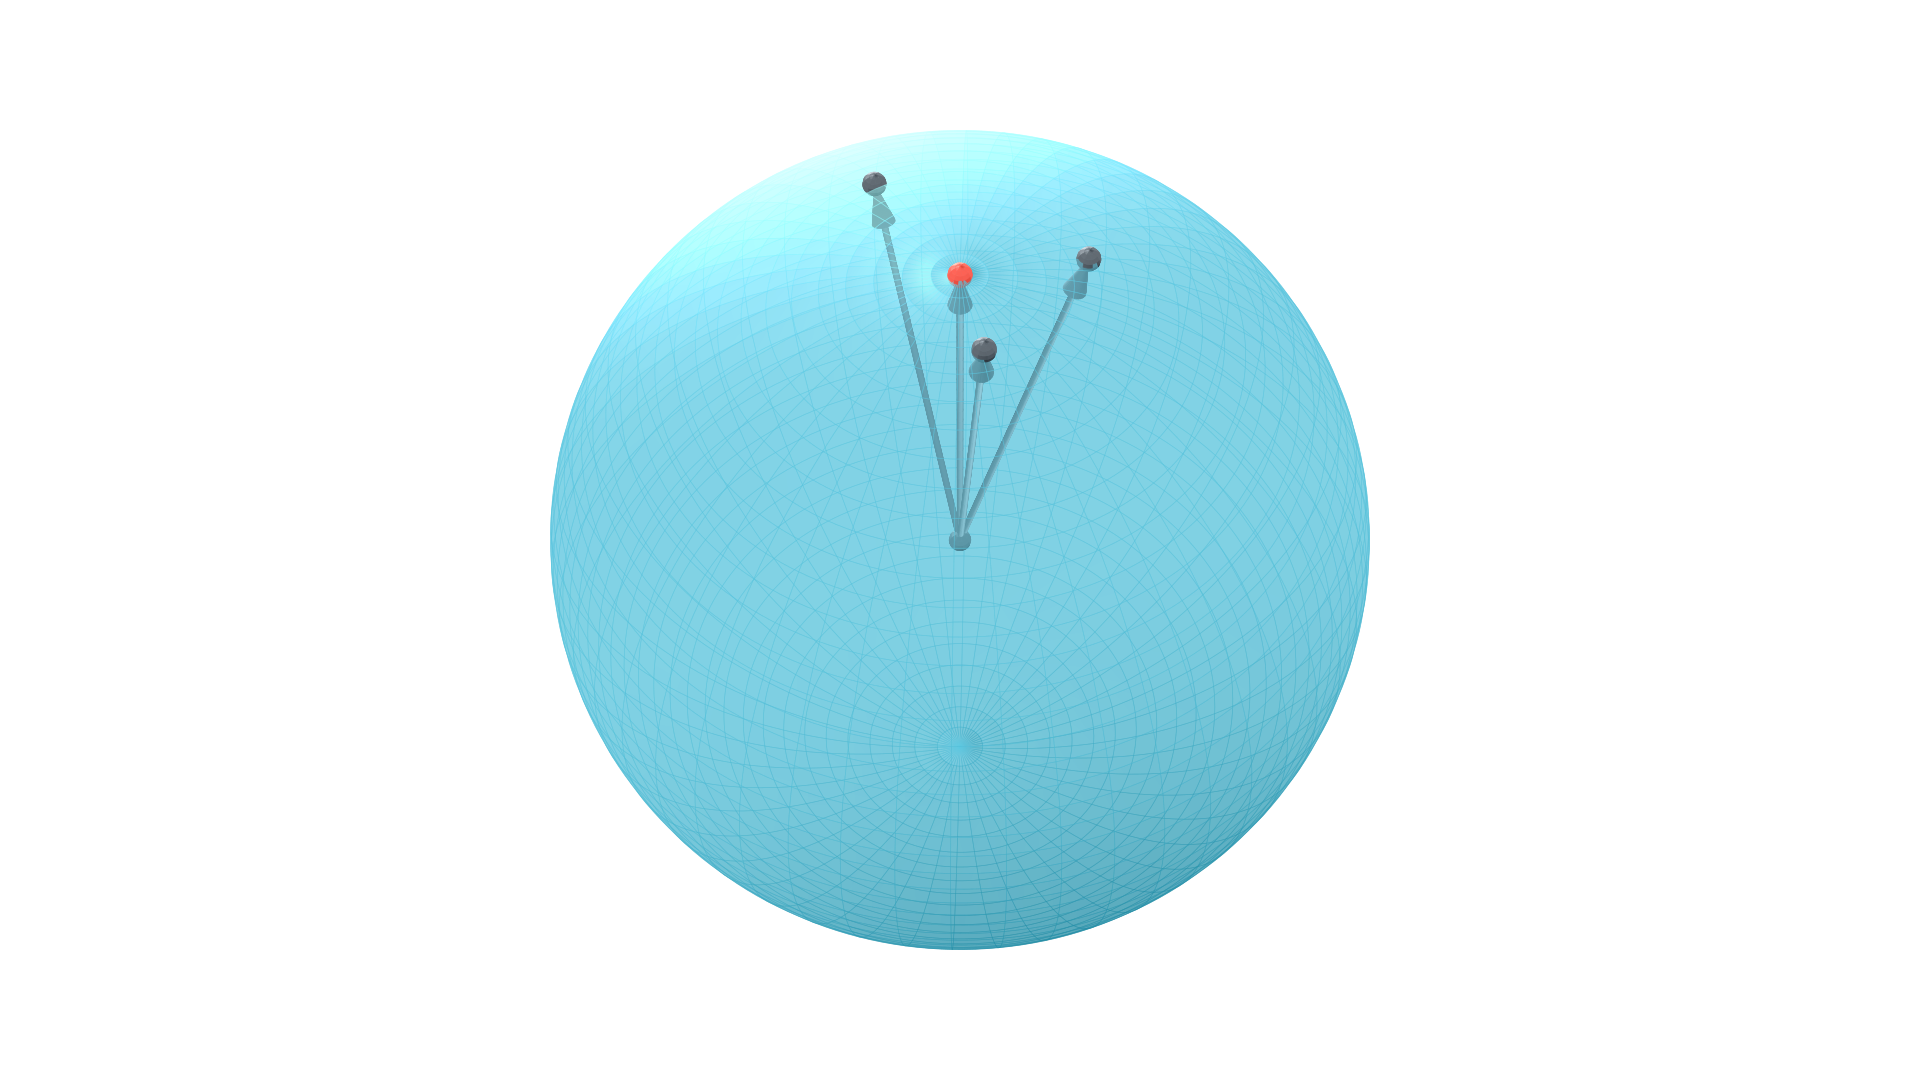
\includegraphics[width=1\textwidth]{media/cmb_sphere_3_ManimCE_v0.17.3.png}
    \end{figure}
\end{frame}

\begin{frame}{Overview of the problem}
    We then define a set of vectors $\vec r_1, \vec r_2, \vec r_3$ where $\vec r_i = \vec x_i - \vec x_0$
    \begin{figure}
        \centering
        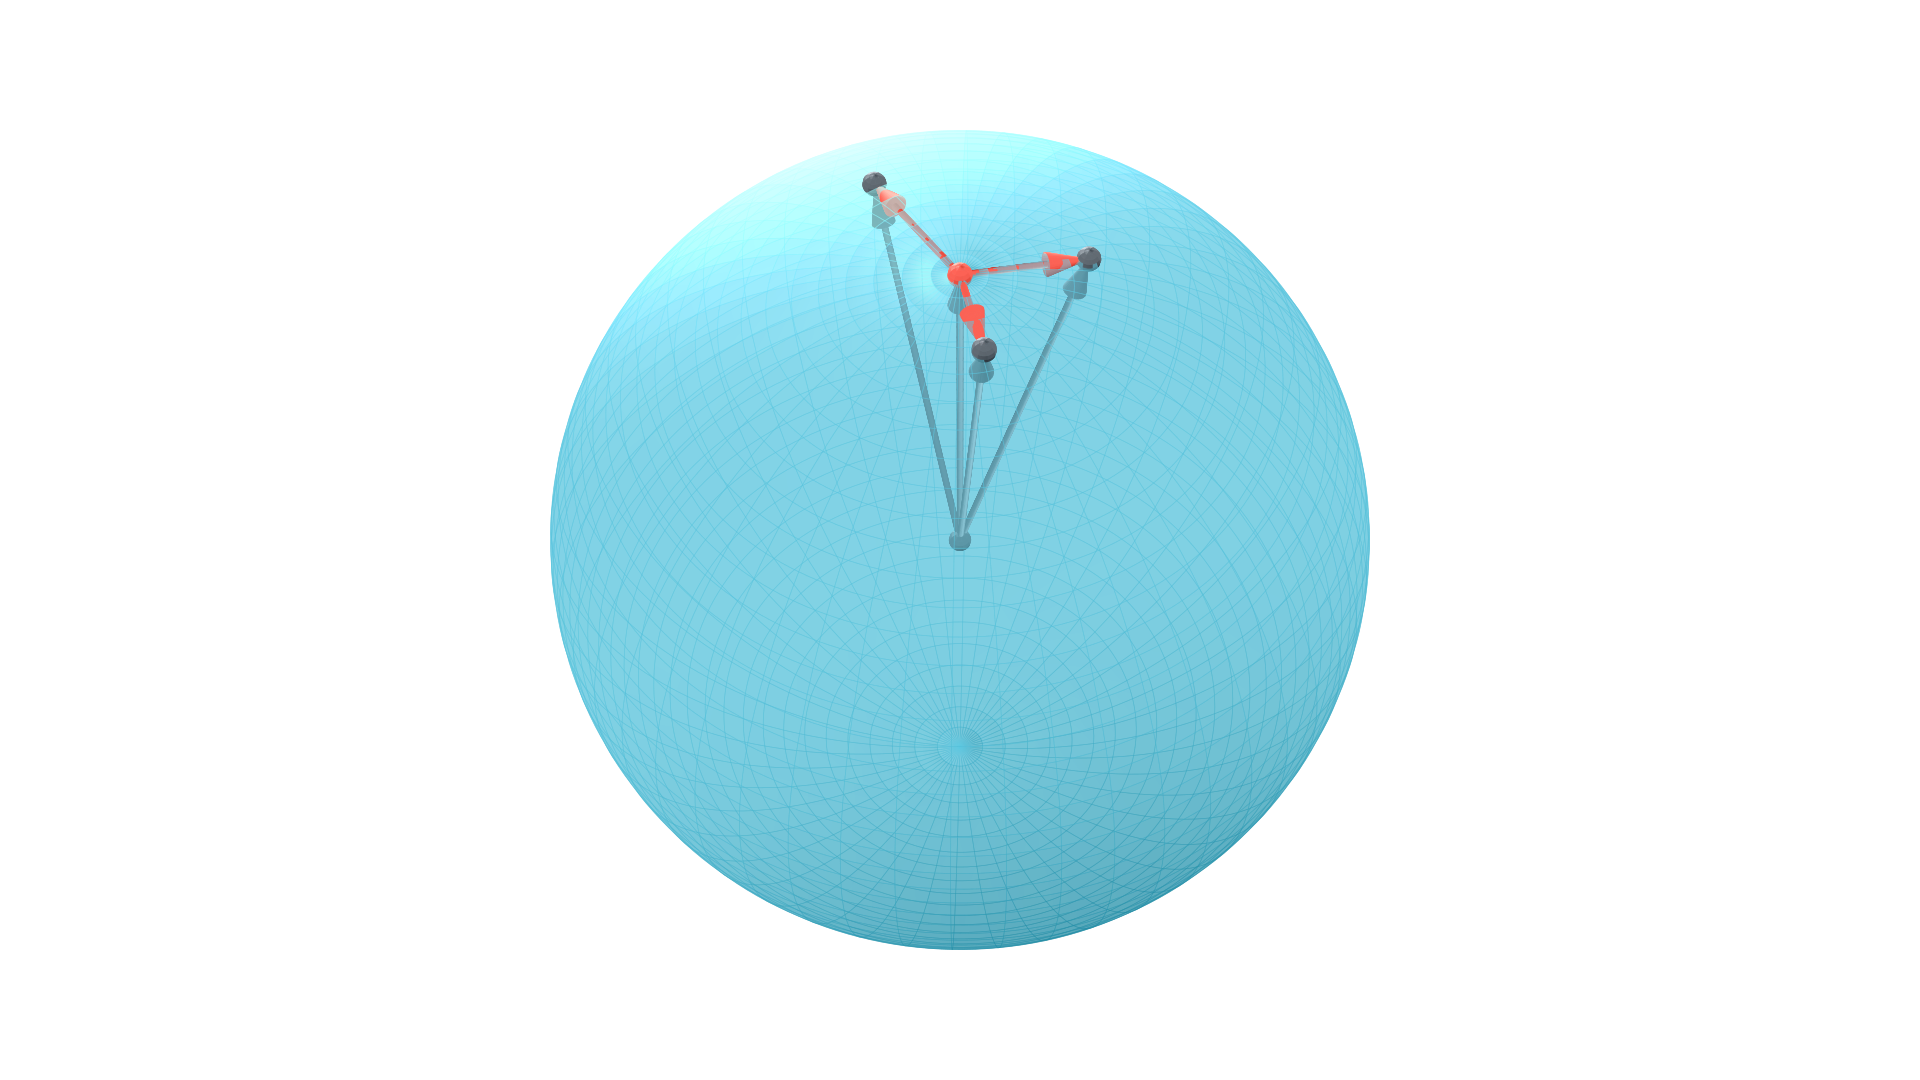
\includegraphics[width=1\textwidth]{media/cmb_sphere_4_ManimCE_v0.17.3.png}
    \end{figure}
\end{frame}

\begin{frame}{Overview of the probelm}
    If we then take two correlation functions:
    \begin{equation*}
        \zeta_E (\vec x_0, \vec x_1, \vec x_2, \vec x_3)
    \end{equation*}
    which is the correlation function of the vectors from the Earth the the CMB and
    \begin{equation*}
        \zeta_{x_0} (\vec r_1, \vec r_2, \vec r_3)
    \end{equation*}
    which is the correlation function centered on point $x_0$, then our goal is to write one as a function of the other
    in order to help constrain the possible parity of both
\end{frame}

\section{Initial Calculations}
    \begin{frame}
        \frametitle{Intitial Calculations}
        Start by expanding the two correlation functions in terms of isotropic basis functions:
        \begin{eqnarray*}
            \zeta_{x_0} (\vec r_1, \vec r_2, \vec r_3) &=& \sum_{\Lambda} {\zeta_{\Lambda}}(r_1, r_2, r_3) \mathcal P_{\Lambda}(\hat r_1, \hat r_2, \hat r_3)\\
            \zeta_E (\vec x_0, \vec x_1, \vec x_2, \vec x_3) &=& \sum_{\Lambda '} {\zeta_{\Lambda '}}(x_0, x_1, x_2, x_3) \mathcal P_{\Lambda '}(\hat x_0, \hat x_1, \hat x_2, \hat x_3)
        \end{eqnarray*}
        Where $\Lambda$ is the set $\{l_1, l_2, l_3\}$ and $\Lambda'$ is the set $\{l_0', l_1', l_{01}', l_2', l_3'\}$
    \end{frame}

    \begin{frame}
        \frametitle{Intitial Calculations}
        We can then set the two functions equal since they are correlation functions describing the same points
        \begin{eqnarray*}
            \zeta_{x_0} (\vec r_1, \vec r_2, \vec r_3) &=& \zeta_E (\vec x_0, \vec x_1, \vec x_2, \vec x_3)\\
            &\Downarrow&\\
            \sum_{\Lambda} \zeta_{\Lambda}(r_1, r_2, r_3) \mathcal P_{\Lambda}(\hat r_1, \hat r_2, \hat r_3) &=& \sum_{\Lambda '} \zeta_{\Lambda '}(x_0, x_1, x_2, x_3) \mathcal P_{\Lambda '}(\hat x_0, \hat x_1, \hat x_2, \hat x_3)
        \end{eqnarray*}
    \end{frame}

    \begin{frame}
        \frametitle{Intitial Calculations}
        We now multiply both sides by $\mathcal P_{\Lambda ''}^*(\hat x_0, \hat x_1, \hat x_2, \hat x_3)$ and then integrate over all orientations
        $d \hat x_0 d \hat x_1 d \hat x_2 d \hat x_3 = d \hat x$
        \begin{eqnarray*}
            \int d \hat x \sum_{\Lambda} \zeta_{\Lambda}(r_1, r_2, r_3) \mathcal P_{\Lambda}(\hat r_1, \hat r_2, \hat r_3) P^*_{\Lambda ''}(\hat x_0, \hat x_1, \hat x_2, \hat x_3) = \\
            \int d \hat x \sum_{\Lambda '} \zeta_{\Lambda '}(x_0, x_1, x_2, x_3) \mathcal P_{\Lambda '}(\hat x_0, \hat x_1, \hat x_2, \hat x_3) P^*_{\Lambda ''}(\hat x_0, \hat x_1, \hat x_2, \hat x_3)
        \end{eqnarray*}
    \end{frame}

    \begin{frame}
        \frametitle{Intitial Calculations}
        Using the orthogonality of isotropic basis functions which states\\
        $$\int d \hat R \ \mathcal P_{\Lambda}(\hat R) \mathcal P^*_{\Lambda'}(\hat R) = \delta_{\Lambda_1 \Lambda_1'}\delta_{\Lambda_2 \Lambda_2'}...$$\\
        we can simplify the right hand side of the previous equation:
        \begin{multline*}
            \int d \hat x \sum_{\Lambda '} \zeta_{\Lambda '}(x_0, x_1, x_2, x_3) \mathcal P_{\Lambda '}(\hat x_0, \hat x_1, \hat x_2, \hat x_3) P_{\Lambda ''}(\hat x_0, \hat x_1, \hat x_2, \hat x_3)\\
            =\zeta_{\Lambda ''}(x_0, x_1, x_2, x_3)
        \end{multline*}
    \end{frame}

    \begin{frame}
        \frametitle{Intitial Calculations}
        Plugging this back into the previous equation we get the key relation:
        \begin{equation}
            \label{main_eq}
            \boxed{\zeta_{\Lambda ''}(x_0, x_1, x_2, x_3) = \int d \hat x \sum_{\Lambda} \zeta_{\Lambda}(r_1, r_2, r_3) \mathcal P_{\Lambda}(\hat r_1, \hat r_2, \hat r_3) P^*_{\Lambda ''}(\hat x_0, \hat x_1, \hat x_2, \hat x_3)}
        \end{equation}
        Solving the integral on the right will
        give an expression for the coefficients of the correlation function centered 
        on earth in terms of the correlation function centered at $x_0$
    \end{frame}

    \section{Solving for Coefficients}

    \begin{frame}
        \frametitle{Solving for $\vec r$ in terms of $\vec x$}
        Consider a great circle going through the poles at an angle $\phi_i$ to the x-axis where
        $\phi_i$ is the $\phi$ angle of vector $\vec x_i$ for $i = 1,2,3$\\
        \begin{figure}
            \centering
                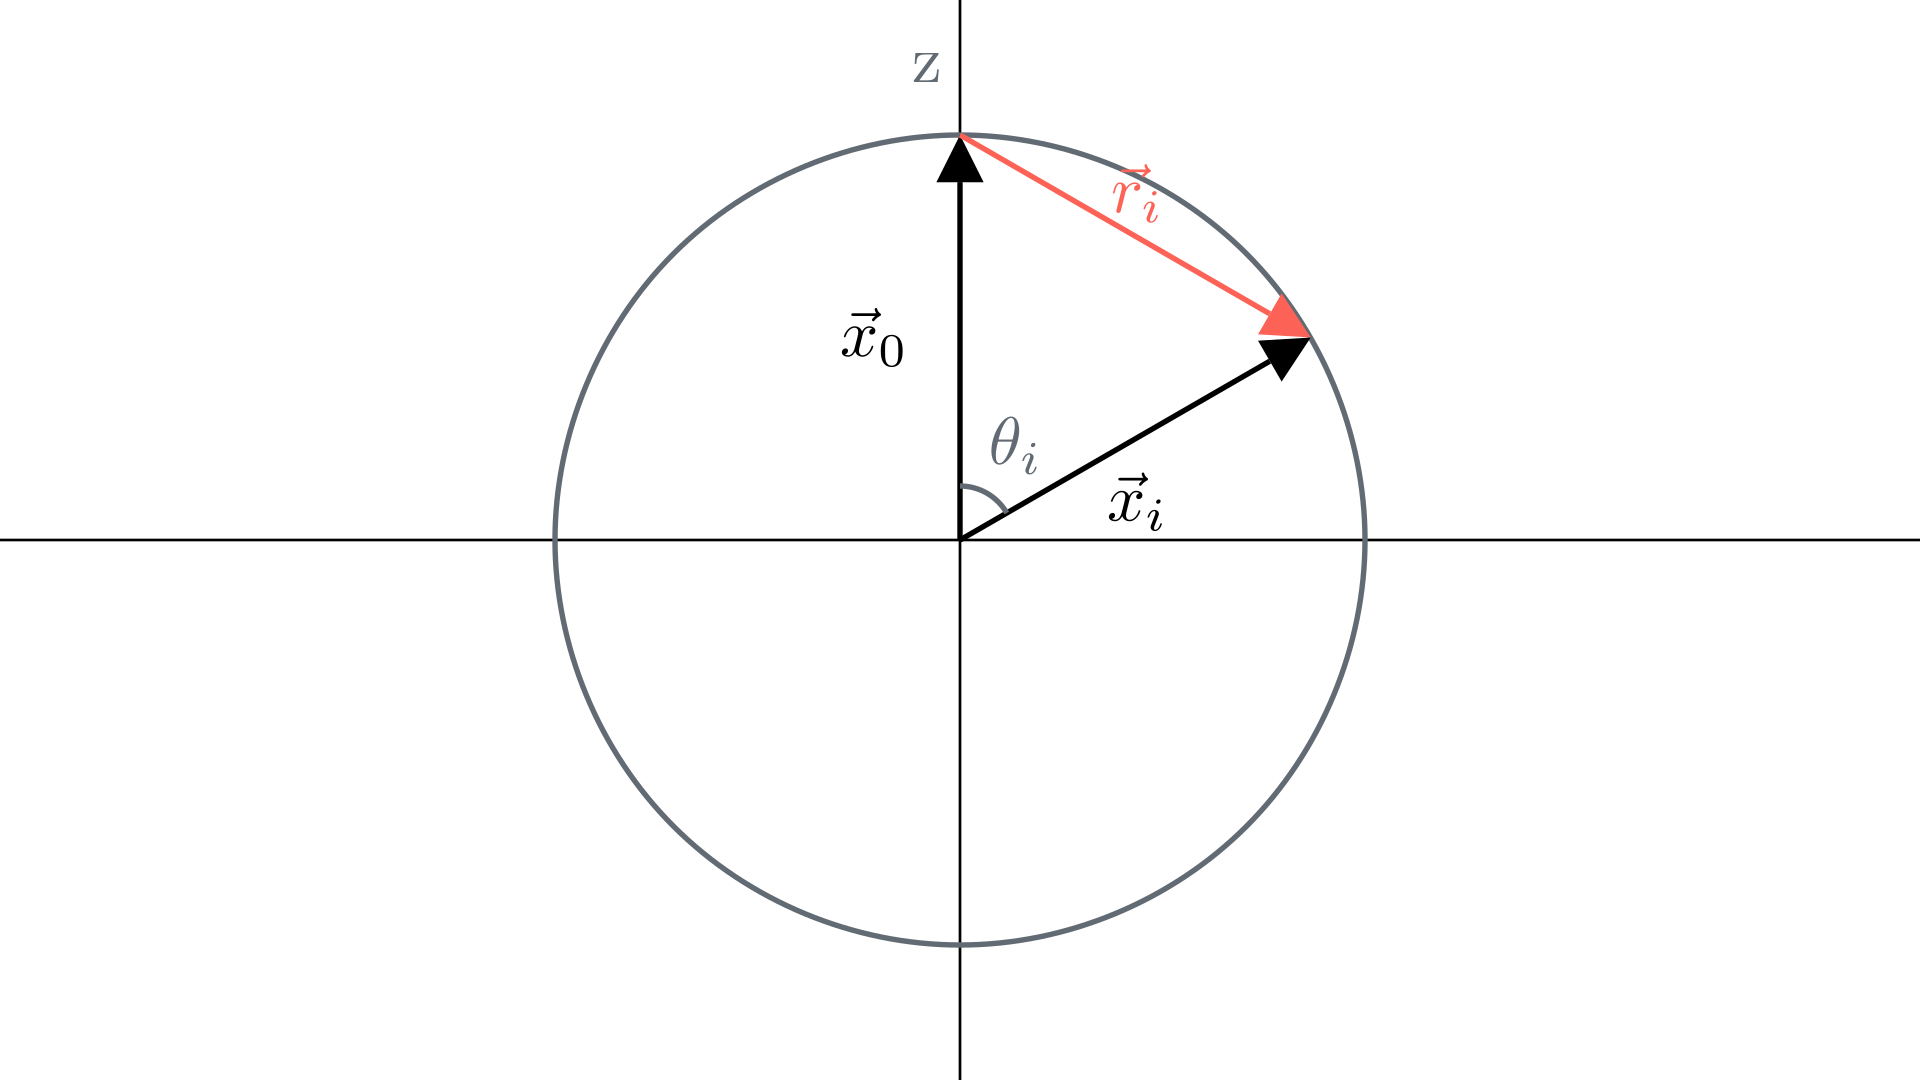
\includegraphics[width=1\textwidth]{media/angle_conversion_diagram_2_ManimCE_v0.17.3.png}
            \end{figure}
    \end{frame}

    \begin{frame}
        \frametitle{Solving for $\vec r$ in terms of $\vec x$}
        Using the law of Cosines and defining the distance to the cmb to be $d^*$ we get:\\
        \begin{equation*}
            |\vec r_i| = \sqrt{d^{*2} + d^{*2} - 2d^*d^*cos(\theta_i)}
        \end{equation*}
        \begin{equation*}
            \boxed{r_i = \sqrt{2}d^*\sqrt{1 - cos(\theta_i)}}
        \end{equation*}

        \begin{figure}
            \centering
                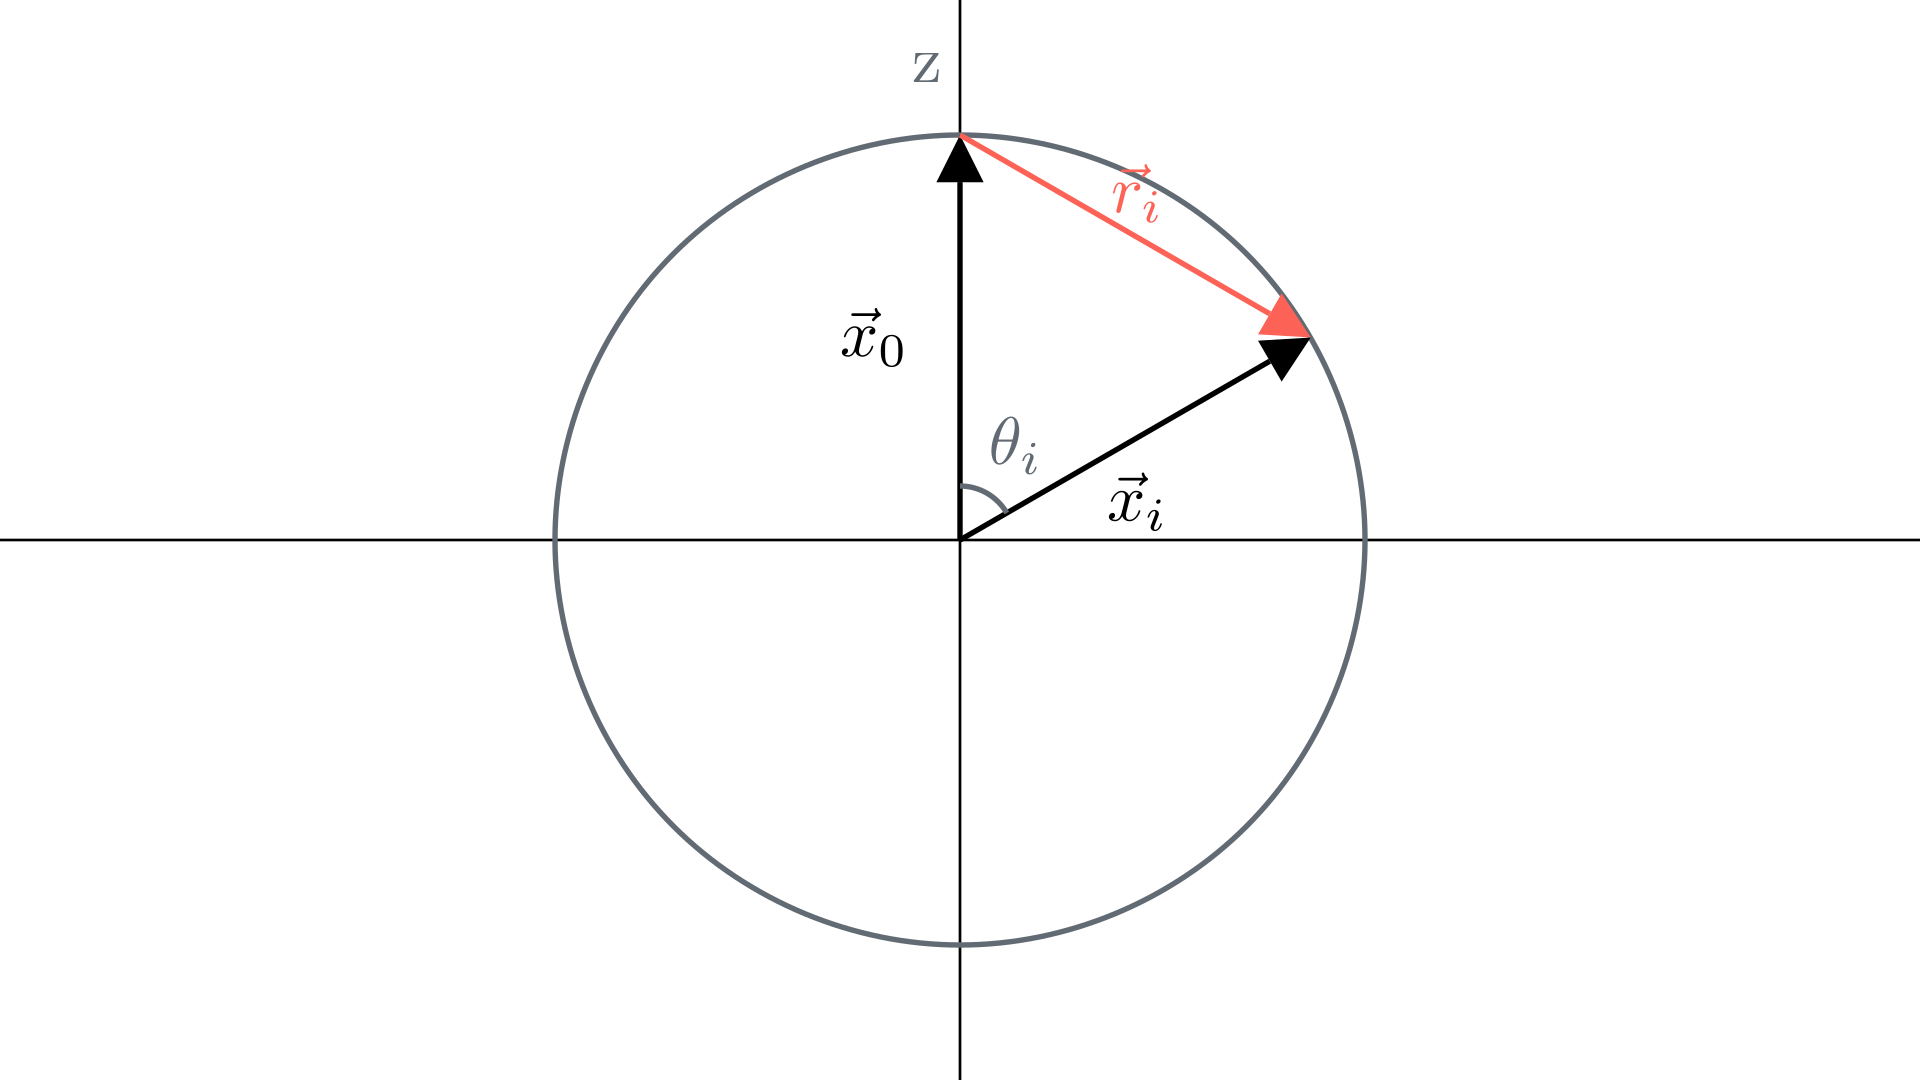
\includegraphics[width=0.8\textwidth]{media/angle_conversion_diagram_2_ManimCE_v0.17.3.png}
            \end{figure}
    \end{frame}

    \begin{frame}
        \frametitle{Solving for $\vec r$ in terms of $\vec x$}
        Similarly, we can solve for the angular dependence of $\vec r_i$\\
        \begin{equation*}
            \boxed{\theta_{ri} = \frac{\pi}{2} + \frac{\theta_i}{2}; \ \phi_{ri} = \phi_i}
        \end{equation*}
        \begin{figure}
            \centering
                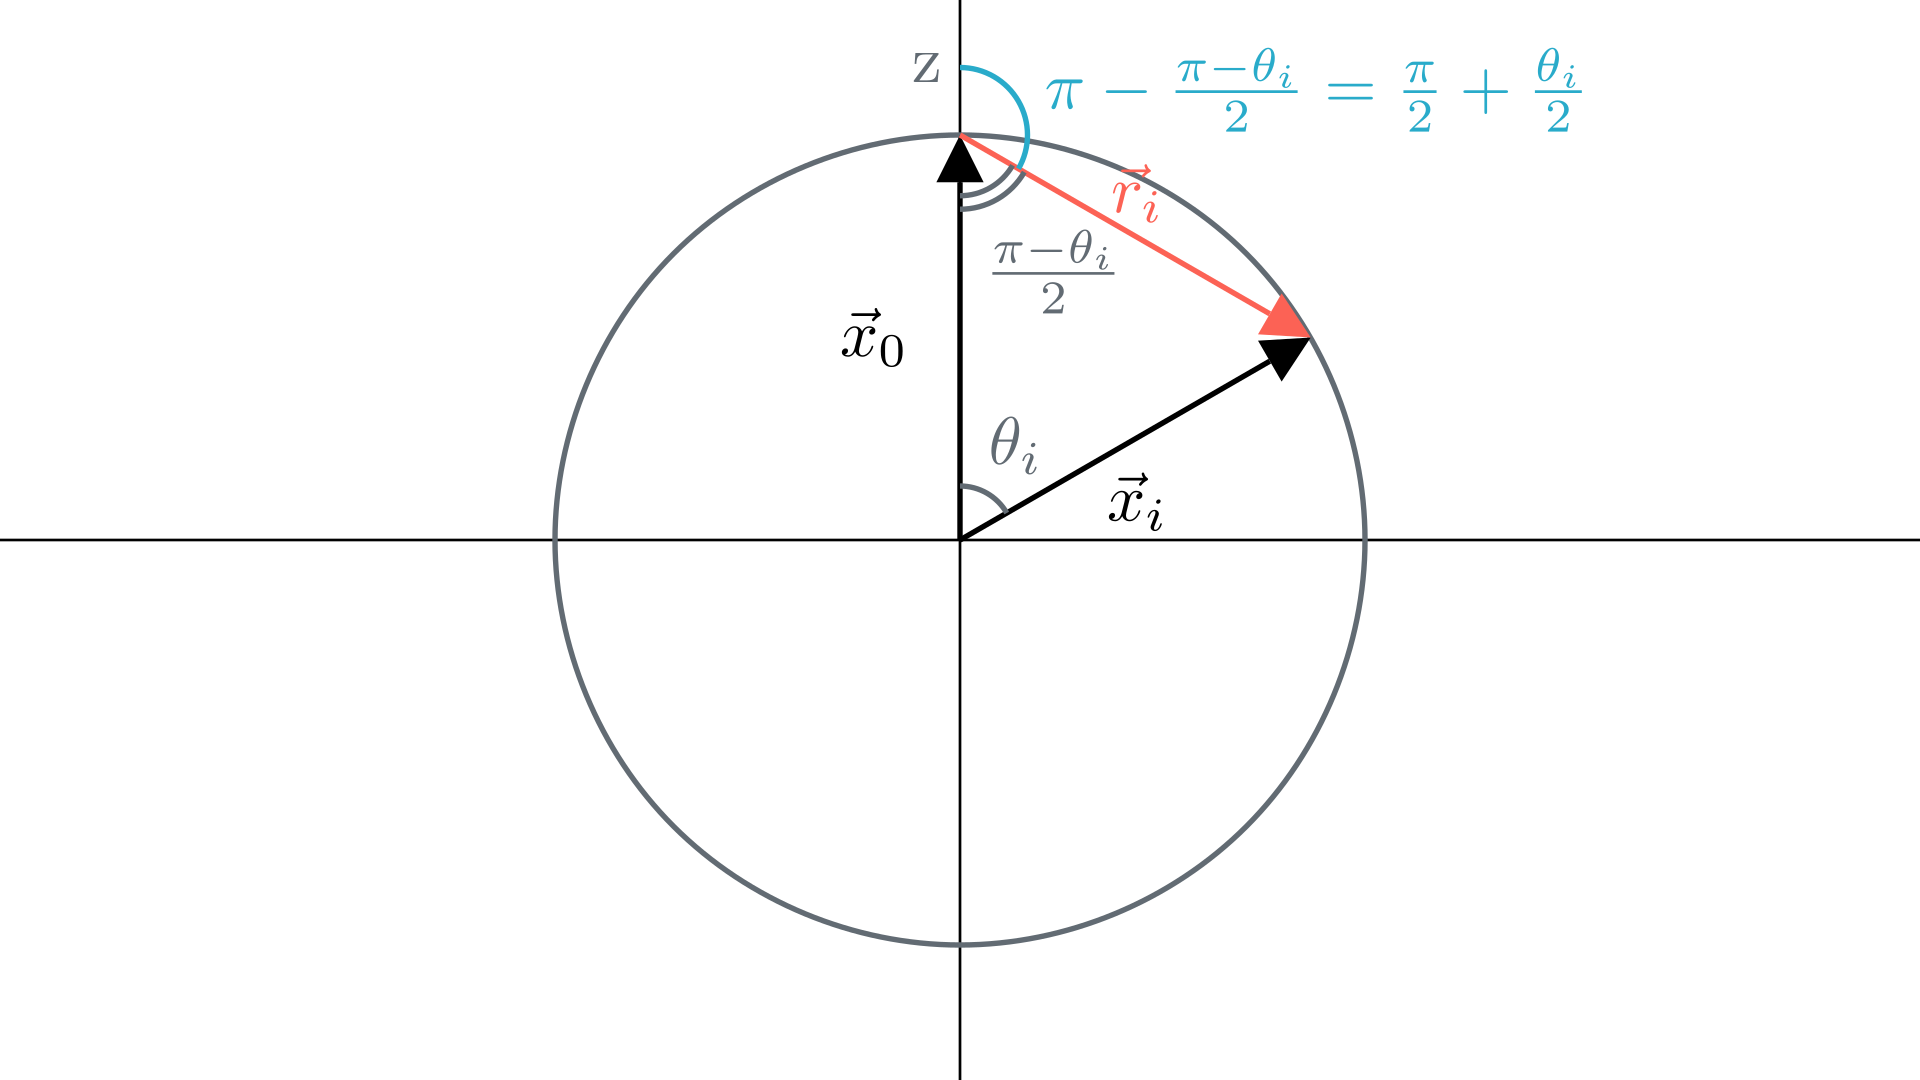
\includegraphics[width=0.9\textwidth]{media/angle_conversion_diagram_1_ManimCE_v0.17.3.png}
            \end{figure}
    \end{frame}

    \begin{frame}
        \frametitle{Solving for the coefficients}
        Plugging those back into equation \ref{main_eq} we get:
        \begin{align*}
            &\zeta_{\Lambda ''}(x_0, x_1, x_2, x_3) =\\
            &\int d \hat x \sum_{\Lambda} \zeta_{\Lambda}(\sqrt{2}d^*\sqrt{1-cos(\theta_1)}, \sqrt{2}d^*\sqrt{1-cos(\theta_2)}, \sqrt{2}d^*\sqrt{1-cos(\theta_3)})\\
            &\times \mathcal P_{\Lambda}(\frac{\pi}{2} + \frac{\theta_1}{2}, \phi_1; \frac{\pi}{2} + \frac{\theta_2}{2}, \phi_2; \frac{\pi}{2} + \frac{\theta_3}{2}, \phi_3)\\
            &\times \mathcal P^*_{\Lambda ''}(\theta_0, \phi_0; \theta_1, \phi_1; \theta_2, \phi_2; \theta_3, \phi_3)
        \end{align*}
    \end{frame}

    \begin{frame}
        \frametitle{Different approaches}
        \begin{itemize}
            \item Directly solving the integral
            \item Rotating the spherical harmonics
            \item Using an addition formula
            \begin{itemize}
                \item Associated Legendre Polynomials
                \item Jacobi Polynomials
            \end{itemize}
        \end{itemize}
    \end{frame}

    \begin{frame}
        \frametitle{Directly solving the integral}
        We can expand the integral using the definitions of the isotropic basis functions:
        \begin{align*}
            &\mathcal P_{l_1 l_2 l_3}(\hat r_1, \hat r_2, \hat r_3) = (-1)^{l_1+l_2+l_3} \sum_{m_1 m_1 m_3} 
            \begin{pmatrix}
            l_1 & l_2 & l_3\\
            m_1 & m_2 & m_3
            \end{pmatrix}\\
            &\times Y_{l_1 m_1}(\hat r_1)Y_{l_2 m_2}(\hat r_2)Y_{l_3 m_3}(\hat r_3)\\ 
            &\\
            &\mathcal P_{l_1 l_2 (l_{12}) l_3 l_4}(\hat r_1, \hat r_2, \hat r_3, \hat r_4) = (-1)^{l_1+l_2+l_3+l_4}\\
            &\times \sum_{m_{12}} (-1)^{l_{12}-m_{12}}
            \sum_{m_1 m_2 m_3 m_4}
            \begin{pmatrix}
                l_1 & l_2 & l_{12}\\
                m_1 & m_2 & -m_{12}
            \end{pmatrix}
            \begin{pmatrix}
                l_{12} & l_3 & l_4\\
                m_{12} & m_3 & -m_4
            \end{pmatrix}\\
            &\times Y_{l_1 m_1}(\hat r_1)Y_{l_2 m_2}(\hat r_2)Y_{l_3 m_3}(\hat r_3)Y_{l_4 m_4}(\hat r_4)
        \end{align*}
    \end{frame}

    \begin{frame}
        \frametitle{Directly solving the integral}
        Looking at just the angular dependent parts of the integral we have:
        \begin{align*}
            &\int d\theta_0 d\phi_0 d\theta_1 d\phi_1 d\theta_2 d\phi_2 d\theta_3 d\phi_3 sin(\theta_0) sin(\theta_1) sin(\theta_2) sin(\theta_3) \\
            &\times \zeta_{\Lambda}(\sqrt{2}d^*\sqrt{1-cos(\theta_1)}, \sqrt{2}d^*\sqrt{1-cos(\theta_2)}, \sqrt{2}d^*\sqrt{1-cos(\theta_3)})\\
            &\times Y_{l'_0 m'_0}(\theta_0, \phi_0) Y_{l'_1 m'_1}(\theta_1, \phi_1) Y_{l'_2 m'_2}(\theta_2, \phi_2) Y_{l'_3 m'_3}(\theta_3, \phi_3) \\
            &\times Y_{l_1 m_1}(\frac{\theta_1}{2} + \frac{\pi}{2}, \phi_1) Y_{l_2 m_2}(\frac{\theta_2}{2} + \frac{\pi}{2}, \phi_2) Y_{l_3 m_3}(\frac{\theta_3}{2} + \frac{\pi}{2}, \phi_3)
        \end{align*}
    \end{frame}

    \begin{frame}
        \frametitle{Directly solving the integral}
        We can further separate the integral into $\phi$ and $\theta$ dependent parts by using the following definition of 
        sperical harmonics:
        \begin{equation*}
            Y_l^m (\theta, \phi) = \sqrt{\frac{2l + 1}{4 \pi} \frac{(l-m)!}{(l+m)!}} P_l^m (cos \theta) e^{im\phi}
        \end{equation*}
    \end{frame}

    \begin{frame}
        \frametitle{Solving the $\phi$ integral}
        Looking at just the $\phi$ dependent terms:
        \begin{align*}
            &\int_0^{2\pi} d\phi_0 d\phi_1 d\phi_2 d\phi_3 e^{im'_0\phi_0}e^{im'_1\phi_1 + im_1\phi_1}e^{im'_2\phi_2 + im_2\phi_2}e^{im'_3\phi_3 + im_3\phi_3}\\
            &= \left[\left.\frac{1}{im'_0}e^{im'_0\phi_0}\right|_0^{2\pi}\right] \prod_j \left[\left.\frac{1}{i(m'_j + m_j)}e^{i(m'_j + m_j)\phi_j}\right|_0^{2\pi}\right]\ for\ j = 1,2,3
        \end{align*}
        Each of the above integrals will always be zero since all m's are integers unless $m'_0 = 0$ and $m'_j + m_j = 0$ in which case
        each term becomes $2\pi$ so the total $\phi$ integral becomes:
        \begin{equation*}
            16\pi^4 \delta^K_{m'_0,0} \delta^K_{m_1,-m'_1} \delta^K_{m_2,-m'_2} \delta^K_{m_3,-m'_3}
        \end{equation*}
    \end{frame}

    \begin{frame}{Examining the 3j symbols}
        Our original expression had three 3j symbols:
        \begin{equation*}
            \begin{pmatrix}
                l'_0 & l'_1 & l'_{01}\\
                m'_0 & m'_1 & -m'_{01}
            \end{pmatrix}
            \begin{pmatrix}
                l'_{01} & l'_2 & l'_{3}\\
                m'_{01} & m'_2 & m'_{3}
            \end{pmatrix}
            \begin{pmatrix}
                l_{1} & l_2 & l_{3}\\
                m_{1} & m_2 & m_{3}
            \end{pmatrix}
        \end{equation*}
        If we now plug in the constraints given by the delta functions from the $\phi$ integral we get:
        \begin{equation*}
            \begin{pmatrix}
                l'_0 & l'_1 & l'_{01}\\
                0 & -m_1 & -m'_{01}
            \end{pmatrix}
            \begin{pmatrix}
                l'_{01} & l'_2 & l'_{3}\\
                m'_{01} & -m_2 & -m_{3}
            \end{pmatrix}
            \begin{pmatrix}
                l_{1} & l_2 & l_{3}\\
                m_{1} & m_2 & m_{3}
            \end{pmatrix}
        \end{equation*}
        Since the bottom elements of the 3j symbol must sum to zero, this adds the additional constraint that $m'_{01}=-m_1$
    \end{frame}

    \begin{frame}{Solving the $\theta$ integral}
        Looking at the $\theta$ integral, we have:
        \begin{align*}
            &\int_0^{\pi} d\theta_0 d\theta_1 d\theta_2 d\theta_3 sin(\theta_0) sin(\theta_1) sin(\theta_2) sin(\theta_3)\\
            &\times \zeta_{\Lambda}(\sqrt{2}d^*\sqrt{1-cos(\theta_1)}, \sqrt{2}d^*\sqrt{1-cos(\theta_2)}, \sqrt{2}d^*\sqrt{1-cos(\theta_3)})\\
            &\times P_{l'_0}^{m'_0}(cos \theta_0) P_{l'_1}^{m'_1}(cos \theta_1) P_{l'_2}^{m'_2}(cos \theta_2) P_{l'_3}^{m'_3}(cos \theta_3) \\
            &\times P_{l_1}^{m_1}(cos (\frac{\theta_1}{2} + \frac{\pi}{2})) P_{l_2}^{m_2}(cos (\frac{\theta_2}{2} + \frac{\pi}{2})) P_{l_3}^{m_3}(cos (\frac{\theta_3}{2} + \frac{\pi}{2}))
        \end{align*}
    \end{frame}

    \begin{frame}{Solving the $\theta$ integral}
        Since $\zeta_{\Lambda}$ is an unknown function, we cannot integrate $\theta_1, \theta_2, \theta_3$ in this form.
        To deal with this we can express $\zeta_{\Lambda}$ as an inverse Fourier Transform leading to:
        \begin{align*}
            &\zeta_{\Lambda}(\sqrt{2}d^*\sqrt{1-cos(\theta_1)}, \sqrt{2}d^*\sqrt{1-cos(\theta_2)}, \sqrt{2}d^*\sqrt{1-cos(\theta_3)})\\
            &= \int dk_1 dk_2 dk_3 j_{l_1}(k_1r_1) j_{l_2}(k_2r_2) j_{l_3}(k_3r_3) \tilde \zeta_{\Lambda}(k1, k2, k3)
        \end{align*}
        Where $j_l$ are the spherical bessel functions of the first kind and $r_i = \sqrt{2}d^*\sqrt{1-cos \theta_i}$
    \end{frame}

    \begin{frame}{Rotating spherical harmonics}
        Another approach to equation \ref{main_eq} is to think of $Y_l^m(\frac{\theta}{2} + \frac{\pi}{2})$ as a rotation of $Y_l^m(\theta)$ by an angle of $\frac{-\theta}{2} + \frac{\pi}{2}$\\
        Using the theorem:
        \begin{equation*}
            Y_l^m(\theta', \phi') = \sum_{m'=-l}^l D_{m'm}^l(R) Y_l^{m'}(\theta, \phi)
        \end{equation*}
        Where $D_{m'm}^l(R)$ is a Wigner D-matrix of some rotation $R$.
    \end{frame}

    \begin{frame}{Rotating spherical harmonics}
        Using the theorem:
        \begin{equation*}
            D_{ms}^l(\alpha, \beta, \gamma) = (-1)^s \sqrt{\frac{4\pi}{2l + 1}} \ _{-s}Y_l^{*m}(\beta, \alpha)e^{-is\gamma}
        \end{equation*}
        we can rewrite the D-matrices as spin-weighted spherical harmonics. When doing this approach however, since we are rotating by $\beta = \frac{-\theta}{2} + \frac{\pi}{2}$
        we still have an argument in terms of $\frac{\theta}{2}$
    \end{frame}

    \begin{frame}{Addition theorems}
        A third approach was inspired by the spherical harmonic addition theorem:
        \begin{equation*}
            P_l(cos(\gamma)) = \frac{4\pi}{2l+1}\sum_{m=-l}^l (-1)^m Y_l^m(\theta_1, \phi_1) Y_l^m(\theta_2, \phi_2)
        \end{equation*}
        where $\gamma$ is the angle between the directions of the $(\theta_1, \phi_1)$ and $(\theta_2, \phi_2)$\\
        If we could find a similar theorem for associated Legendre polynomials, we may be able change the form of $P_l^m(cos(\frac{\theta/2}{2} + \frac{\pi}{2}))$
        into different form.
    \end{frame}

    \begin{frame}{Addition theorems}
        B. E. Johnson (1964) proposed an addition theorem for associated Legendre polynomials, however, the domain of his function only includes real values greater than 0, which is
        not necessarily true for $cos(\frac{\theta/2}{2} + \frac{\pi}{2})$\\
        Similarly, Koornwinder (1973) gives an addition theorem for Jacobi polynomials, however, we don't believe associated Legendre polynomials are a special case of Jacobi polynomials
    \end{frame}
        
    \section{Further Work}

    \begin{frame}{Further Work}
        \begin{itemize}
            \item We assumed we can set $\hat x_0 = \hat z$, however, we then integrate over $\hat x_0$
            \begin{itemize}
                \item Define a rotation from absolute to relative coordiates $R\hat x_0 = \hat z$
                \item How does this impact the integral?
            \end{itemize}
            \item How do we solve the $\theta$ integral?
            \item Can we derive more information from the 3j symbols?
        \end{itemize}

    \end{frame}
\end{document}
